\documentclass[12pt]{article}
\usepackage{amsmath,amsfonts,bm}
\usepackage[bookmarks, colorlinks=TRUE, linkcolor=blue, urlcolor=red,
citecolor=black, pdftitle={amer: Using lme4 to fit Generalized Additive Mixed
Models}, pdfauthor={Fabian Scheipl}]{hyperref}
\usepackage[authoryear,round]{natbib}
\bibliographystyle{plainnat}
\usepackage{framed}

% instead of \usepackage{Sweave}
\RequirePackage[T1]{fontenc}
\RequirePackage{graphicx,ae,fancyvrb} 
\IfFileExists{upquote.sty}{\RequirePackage{upquote}}{} 
\setkeys{Gin}{width=0.8\textwidth} 
\DefineVerbatimEnvironment{Sinput}{Verbatim}
{formatcom={\vspace{-1ex}},fontshape=sl,
  fontfamily=courier,fontseries=b, fontsize=\footnotesize}
\DefineVerbatimEnvironment{Soutput}{Verbatim}
{formatcom={\vspace{-1ex}},fontfamily=courier,fontseries=b,%
  fontsize=\footnotesize}
\newenvironment{Schunk}{}{} 
\setkeys{Gin}{width=\textwidth}

\parskip 9pt


% envs
\newcommand{\code}[1]{\texttt{\small{#1}}}
\newcommand{\package}[1]{\textsf{\small{#1}}}
\newcommand{\bvec}{\left[\begin{array}{c}}
\newcommand{\evec}{\end{array}\right]}
\newcommand{\bmat}[1]{\left[\begin{array}{*{#1}{c}}}
\newcommand{\emat}{\end{array}\right]}

%symbols
\newcommand{\ra}{\rightarrow}
\newcommand{\Ra}{\Rightarrow}
\newcommand{\lra}{\Leftrightarrow}
\newcommand{\im}{\item}
\newcommand{\tr}{^\prime}
\newcommand{\eps}{\varepsilon}
\newcommand{\R}{\textsf{R}}
\newcommand{\sigmaeps} {\sigma^2_{\eps}}

%operators
\newcommand{\iid} {\operatorname{i.i.d.}}
\newcommand{\Var}{\operatorname{Var}}
\newcommand{\Cov}{\operatorname{Cov}}
\newcommand{\mean}{\operatorname{mean}}
\newcommand{\diag} {\operatorname{diag}}
\newcommand{\blockdiag}{\operatorname{blockdiag}}

%<<cacheSweave, echo=F, results=hide>>=
%library(cacheSweave)
%setCacheDir("F:/lme4Spline/amer/inst/doc")	
%@
%<<setwd, echo=F, results=hide>>=
%setwd("~/RegularBayes/Workspace/amer/amer/inst/doc")	
%@


%\VignetteIndexEntry{amer - GAMMs with lme4}

\begin{document}

\title{ \textsf{amer}: Using \textsf{lme4} to fit Generalized Additive Mixed Models}
\author{Fabian Scheipl\footnote{\texttt{fabian.scheipl@stat.uni-muenchen.de}} \\ LMU M�nchen}

\maketitle

\begin{abstract}
  The \package{lme4} package uses sparse matrix technology and clever decompositions of the  like\-lihood 
  to fit linear, generalized, and nonlinear mixed-effects models.  The \package{amer} package extends 
  \package{lme4}'s scope to include generalized \emph{additive} mixed models (GAMM). 
  This vignette summarizes the main ideas behind additive models and their representation in the form of a mixed model,
  describes the modifications to \code{lmer} necessary for fitting GAMMs and presents some examples with real data.
\end{abstract}
\newpage

\tableofcontents
\newpage

\section{Additive Models}
In many applications, the assumption of a linear dependence of the
response on predictor variables is inappropriate. Modelling smooth
functions of an unknown shape, that is, models of the form
\[
\bm y=\sum_{s=1}^S f_s(\bm x_s) +\bm\eps;\quad \bm\eps\sim N_n(0,\sigmaeps \bm I_n)
\]
where $f_s(\cdot)$ is some smooth function of a covariate $\bm x_i$,
which can also be multidimensional (e.g. surface estimation), requires solving 3 problems not
encountered in linear modelling:
\begin{enumerate}
	\item the smooth function has to be represented somehow
	\item the degree of smoothness of the function must be controllable
	\item the appropriate degree of smoothness should be selected
in a data-driven way
\end{enumerate}

Spline smoothing addresses the first issue by assuming that $f_s(\bm x_s)$
can be approximated by a linear
combination of $d_s$ basis functions $B_j(\bm x_s),\; j =1,\dots,d_s$: 
\[
f_s(\bm x_s) \approx \bm B_s \bm \delta_s; \quad \bm B_s=\bmat{3} B_1(x_{s1}) & \hdots &
B_{d_s}(x_{s1}) \\ \vdots & & \vdots \\B_1(x_{sn}) & \hdots &
B_{d_s}(x_{sn}) \emat
\]
This obviously leads back to a linear modelling context. 
For ease of notation we set $S=1$ and drop the subscript $s$ in the following.

The second issue, controlling the roughness or ``wiggliness'' of the
estimated function, is a variant of the bias-variance tradeoff
problem: using too few basis functions may
not allow the fitted curve to accurately represent the shape of the
function, leading to biased estimation, while using too many will result
in an overly close interpolation of the data --- the estimated curve represents 
random noise along with the underlying structure.
Penalized spline smoothing \citep{Eilers:Marx:1996} addresses this problem by
choosing a sufficient number of knots (e.g. 10-40) to ensure the necessary
flexibility of the fit and by introducing an additional penalty term, a function
of the spline coefficients $\bm \delta$, that quantifies the roughness of the
estimated function. For a broad class of spline bases, the resulting criterion is
a penalized least squares criterion,
\begin{eqnarray}\label{F:PenLScriterion}
\underset{\bm \delta}{\operatorname{min
}}\left(\|\bm{y-B\delta}\|^2+\frac{1}{\lambda}\bm{\delta\tr K \delta} \right),
\end{eqnarray}
where $\bm{K}$ is a penalty matrix and $\lambda$ is the smoothing parameter
controlling the amount of penalization, i.e. the tradeoff between fidelity to the
data and complexity of the fit. The elements in $\bm K$ are determined by the
spline basis that is used to generate $\bm B$ and the roughness penalty desired
by the analyst (usually penalizing (local) deviations of the fitted function from
a constant, linear, or a quadratic polynomial). 

\begin{center}
\fbox{ 
\begin{minipage}{.95\textwidth} \noindent
\textbf{Example: TP-Basis}\\
A simple example of basis functions is the truncated powers (TP) basis. A
TP-Basis of degree $p$, with $d$ basis functions for a covariate $\bm x$ and
fixed knots $\kappa_1, \dots, \kappa_{d-p}$ consists of a constant term, $p$
global polynomial terms  $\bm x^1, \dots,\bm x^p$ and $p-d$ truncated polynomials 
$(\bm x- \kappa_i)_+^p,\; i=1,\dots,d-p$, where $(y)_+ = y\, I(y>0)$: $$\bm B =
\bmat{7} \bm x^0 &\bm x^1 &\hdots & \bm x^p &  (\bm x- \kappa_1)_+^p & \hdots &
(\bm x- \kappa_{d-p})_+^p \emat$$ The penalty for the TP-Basis penalizes
deviations of the fitted function from a $p$-degree polynomial: $$\bm K =
\diag(\bm 0_{p+1}, \bm 1_{d-p}).$$ The penalty term $\bm{\delta\tr K \delta}$ is
simply the sum of squares of the $p-d$ coefficients for the truncated
polynomials.
\end{minipage}}
\end{center}



\section{Mixed model representation of an additive model} 

\subsection{Reparameterization: Separating penalized and unpenalized components of smooth terms}\label{Reparam}

The third issue -- selecting the appropriate smoothness in a
data-driven way -- then reduces to estimation of the smoothing parameter $\lambda$,
which controls the smoothness of the estimated function. The penalized least
squares problem is reformulated as a mixed model in which the smoothing parameter
becomes a variance component. This is achieved by a decomposition of the spline
coefficients into an unpenalized part and a penalized part: 
	\[ \bm \delta= \bm{U\beta} + \bm{Pb} \] 
where $\bm U$, $d \times p$, is a basis of the
$p$-dimensional nullspace of the penalization matrix $\bm K$ and $\bm U$ and
$\bm P$ have the following properties \citep[ch. 5.1]{Kneib:06}:
\begin{enumerate}
\item The matrix $[\bm U \bm P]$ has full rank to make the
transformation above a one-to-one transformation. This also implies that both
$\bm U$ and  $\bm P$ have full column rank.
\item  $\bm U$ and  $\bm P$ are orthogonal, i. e. $\bm U \bm P\tr = \bm 0$
\item $\bm{U\tr KU} = \bm 0 $, so that $\bm \beta$ is unpenalized by $\bm K$
\item $\bm{P\tr KP} = \bm I$, so that the penalty for $\bm b$ reduces to $\|\bm b\|^2$
\end{enumerate}
The decomposition is not unique, but it can always be based on the spectral
decomposition of $\bm K$. With
 $$\bm K = [\bm{ \Lambda_+  \Lambda_0}]\tr \bmat{2} \bm{\Gamma_+} & \bm 0 \\ \bm
 0 & \bm 0\emat [\bm{ \Lambda_+  \Lambda_0}],$$
where $\bm \Lambda_+$ is the matrix of the eigenvectors associated with the
positive eigenvalues $\diag(\bm{\Gamma_+})$, and $\bm \Lambda_0$ are the
eigenvectors associated with the zero eigenvalues, the decomposition is
\begin{align*}
\bm{U} &= \bm \Lambda_0, \\
\bm{P} &= \bm L(\bm{L\tr L})^{-1} 
\end{align*}
with $\bm{L} = \bm \Lambda_+ \bm{\Gamma_+}^{1/2}$.


Using
\begin{eqnarray}\label{F:Reparam}
\bm{B\delta} &=& \bm B( \bm{U\beta} + \bm{Pb} )=\bm{X_u\beta} + \bm{Z_p b} \\
\mbox{and}\quad \bm {\delta\tr K \delta} &=& (\bm{U\beta} + \bm{Pb})\tr \bm K(\bm{U\beta} + \bm{Pb}) = \bm{ b\tr b}, \nonumber
\end{eqnarray}
the penalized least squares criterion (\ref{F:PenLScriterion}) can
be rewritten as
\begin{eqnarray}
\underset{\delta}{\operatorname{min
}}\left(\|\bm y- \bm{B\delta}\|^2+ \frac{1}{\lambda} \bm{\delta\tr K \delta}  \right) &=& \label{F:PenLScrit2}\\
&& \underset{\beta, b}{\operatorname{min}}\left(\|\bm y- \bm{X_u\beta}-\bm{Z_p b}\|^2+\frac{1}{\lambda}\|\bm b\|^2\right) \nonumber 
.
\end{eqnarray} 
For given $\lambda$, minimizing \eqref{F:PenLScrit2} over
$(\bm{\beta\tr,b\tr})\tr$ is equivalent to BLUP-estimation \cite[ch.
4.5.3]{Semip:Regr} in a linear mixed model with
\[
\bm y= \bm{X_u\beta} + \bm{Z_p b}+ \bm \eps;\quad  \bm \eps\sim N_n(0,\sigmaeps  \bm{I_n}); \quad
\bm b\sim N_{d-p}(0, \sigmaeps\lambda \bm I_{d-p}),
\]
which means maximizing
\begin{eqnarray*}
L(\bm{\beta,b}|\lambda,\sigmaeps) &\propto& 
\exp\left(\frac{\|\bm y- \bm{X_u\beta} - \bm{Z_p b}\|^2+\frac{1}{\lambda}\|\bm{b}\|^2}{-2\sigmaeps}\right).
\end{eqnarray*}
The reformulation of the additive model as a mixed model therefore makes it possible to estimate 
smoothing parameters with ML- or REML-methodology. 
All this is valid for non-gaussian responses as well.

\subsection{Additive mixed models}

This model formulation can be extended to include
multiple smooth terms, other random effects and a linear predictor
in the classical sense of linear regression: 
Just concatenate the unpenalized parts of
the smooth terms to the design matrix of the fixed effects and the
penalized parts of the smooth effects to the design matrix of the
random effects.\\
For an additive mixed model
\[
\bm y= \bm{X\beta} + \sum^L_{l=1}\bm{Z_l b_l} +\sum_{s=1}^S f(\bm x_s)+\eps;\quad \bvec \bm b \\
\bm \eps \evec \sim N_{\sum q_l + n}\left(\bm 0,\sigmaeps \bmat{2} \Omega_b^{-1} & 0 \\
0 & I_n \emat \right)
\]
with fixed effects design $\bm X$, $L$ random effects designs $\bm Z_l$ each with
$q_l$ parameters and random effects 
$\bm b=[\bm b_1,\dots,\bm  b_L] \sim N_{\sum q_l}(\bm 0, \sigmaeps\Omega_b^{-1})$
and $S$ smooth terms, we can write
\[
\bm y= \bm {\tilde X \tilde \beta + \tilde Z \tilde b + \eps}
\]
with concatenated design matrices
\begin{eqnarray*}
&& \bm{\tilde X}=\left[ \bm{X} \bm{X}_{u,1} \hdots \bm{X}_{u,S}\right];\quad
 \bm{\tilde Z}=\left[ \bm{Z}_1 \hdots \bm{Z}_L \bm{Z}_{p,1} \hdots \bm{Z}_{p,S} \right] \\
&&
\text{and} \quad \Cov(\bm{\tilde b})= \Cov \left( \bvec \bm b \\ \bm b_1 \\ \vdots \\
\bm b_S \evec \right) =
\sigmaeps \bmat{4} \bm \Omega_b^{-1}& 0 & \hdots & 0 \\ 0&\lambda_1 \bm I_{d_1-p_1}&  &\vdots \\
                  \vdots &  &\ddots&0\\0&\hdots&0&\lambda_s \bm I_{d_S-p_S} \emat
\end{eqnarray*}
The parameter vector for the fixed effects is stacked in the same fashion as the
one for the random effects. A minor additional complication arises from the fact
that usually every matrix $\bm X_{u,s},\,s=1,\dots,S$ for the unpenalized part
of the various smooth terms will contain an intercept column. These are dropped in order %%% REWRITE THIS!!
to avoid a rank deficient design matrix $\bm{\tilde X}$. This also solves the
identifiability issues common to additive models \cite[ch. 3.3]{Wood:2006} 
-- in this parameterization, the smooth functions etc. represent
deviations from a global intercept.

\subsection{Variability Estimation}\label{VarEst} 
The convenience functions \code{getF} and \code{plotF} to extract or plot
estimated function values $\hat f(x)$ offer both MCMC-based or approximate
frequentist variability bands. MCMC-based intervals (option
\code{interval="MCMC"} in \code{getF, plotF}) are pointwise HPD-intervals. They
are based on samples from \package{lme4}'s \code{mcmcsamp} and may not be very
reliable yet.\footnote{You can check the traceplots by calling \newline
\texttt{xyplot(attr(getF(<MyModel>, interval="MCMC"),"mcmc"))},\newline see section
\ref{VarBands} for an example.}

The frequentist variability estimates (option \code{interval="RW"} in \code{getF,
plotF}) condition on the value of the estimated variance / smoothing parameters
and use the bias-adjusted covariance of $\hat f(x)$ derived in \citet[ch. 6.4,
eq. (6.13)]{Semip:Regr}. See section \ref{VarBands} for an example. I plan to
include bootstrap-based variability estimates in a future version.

%% add profile confints as soon as lme4a is released.

\clearpage
\section{Examples}\label{Examples}
Let's fit models to some exemplary datasets to show what \code{amer} can do.
I demonstrate how to fit simple semiparametric or additive
models (\ref{ExGAM}), how to use the \code{by}-option of the basis-generating function to fit
group-specific smooths (\ref{ExBy}), how to use the \code{allPen}-option of the
basis-generating function to fit subject- or cluster-specific smooth terms where
all subject-level coefficients are penalized (i.e. the coefficients associated
with $\bm X_u$ are treated as random effects as well) (\ref{ExAllP}), and how to use the
\code{varying}-option to fit varying-coefficient models (\ref{ExVCM}). 
Most of the examples are adapted from \cite{Crainiceanu:2005}. 
Many additional examples on artificial data can be found in the subdirectory \code{tests} 
of the package.

\subsection{Generalized Additive Model}\label{ExGAM}
Let's first have a look at data on wages and union membership for 534 workers
described in \citet{Berndt:1991}. The model assumes that the probability of union
membership of worker $i$ ($y_i=1$ if member) depends on his or her hourly wages
$x_i$. The smooth function is represented by a linear TP-basis:
\begin{align*}
P(y_i=1) &= \operatorname{logit}^{-1}(f(x_i))\\
f(x_i) &= \beta_0 + \beta_1 x_i + \sum_{k=1}^{K-1}  b_k(x_i- \kappa_k)_+\\
b_k &\sim N(0, \sigma^2_f) 
\end{align*}
We use a the default number of basis function
($K=15$) and degree by calling the \code{tp}-function:
\begin{Schunk}
\begin{Sinput}
> data(union)
> u1 <- amer(UNION ~ tp(WAGE), family = binomial, data = union)
\end{Sinput}
\end{Schunk}
By default, \code{tp} uses quantile-based knot spacing to generate the basis functions. If the covariate distribution is 
as non-uniform as here (see figure \ref{unionPlot}), these are often a better choice than equidistant knots.

\begin{Schunk}
\begin{Sinput}
> print(u1, corr = F)
\end{Sinput}
\begin{Soutput}
Generalized additive mixed model fit by the Laplace approximation 
Formula: UNION ~ tp(WAGE) 
   Data: union 
 AIC BIC logLik deviance
 483 496   -238      477
Random effects:
 Groups Name Variance Std.Dev.
 f.WAGE tp   0.200    0.448   
Number of obs: 534, groups: f.WAGE, 14

Fixed effects:
            Estimate Std. Error z value Pr(>|z|)  
(Intercept)   -0.961      0.759   -1.27    0.206  
WAGE.fx1       1.841      0.917    2.01    0.045 *
---
Signif. codes:  0 '***' 0.001 '**' 0.01 '*' 0.05 '.' 0.1 ' ' 1 
\end{Soutput}
\end{Schunk}
Note \code{amer}'s naming convention for the smooth function: The group name of
the variance component associated with a smooth function of a covariate \code{x}
is \code{f.x}, instead of the covariate name, \code{amer} gives the name of the
basis generating function. The names of the columns in the $n \times p$ design
matrix $\bm X_u$ for the unpenalized part of the smooth are given by \code{x.fx1,
x.fx2} to \code{x.fxp}. We see that $\hat \sigma^2_f \approx$ 0.2.
Figure \ref{unionPlot} shows the plot produced by a call to \code{plotF}.
\begin{figure}[!htbp]
\begin{center}
\begin{Schunk}
\begin{Sinput}
> plotF(u1, trans = plogis, rug = F, ylim = c(0, 0.4))
> with(union, points(WAGE, jitter(0.4 * UNION, factor = 0.15), 
+     cex = 0.5))
\end{Sinput}
\end{Schunk}
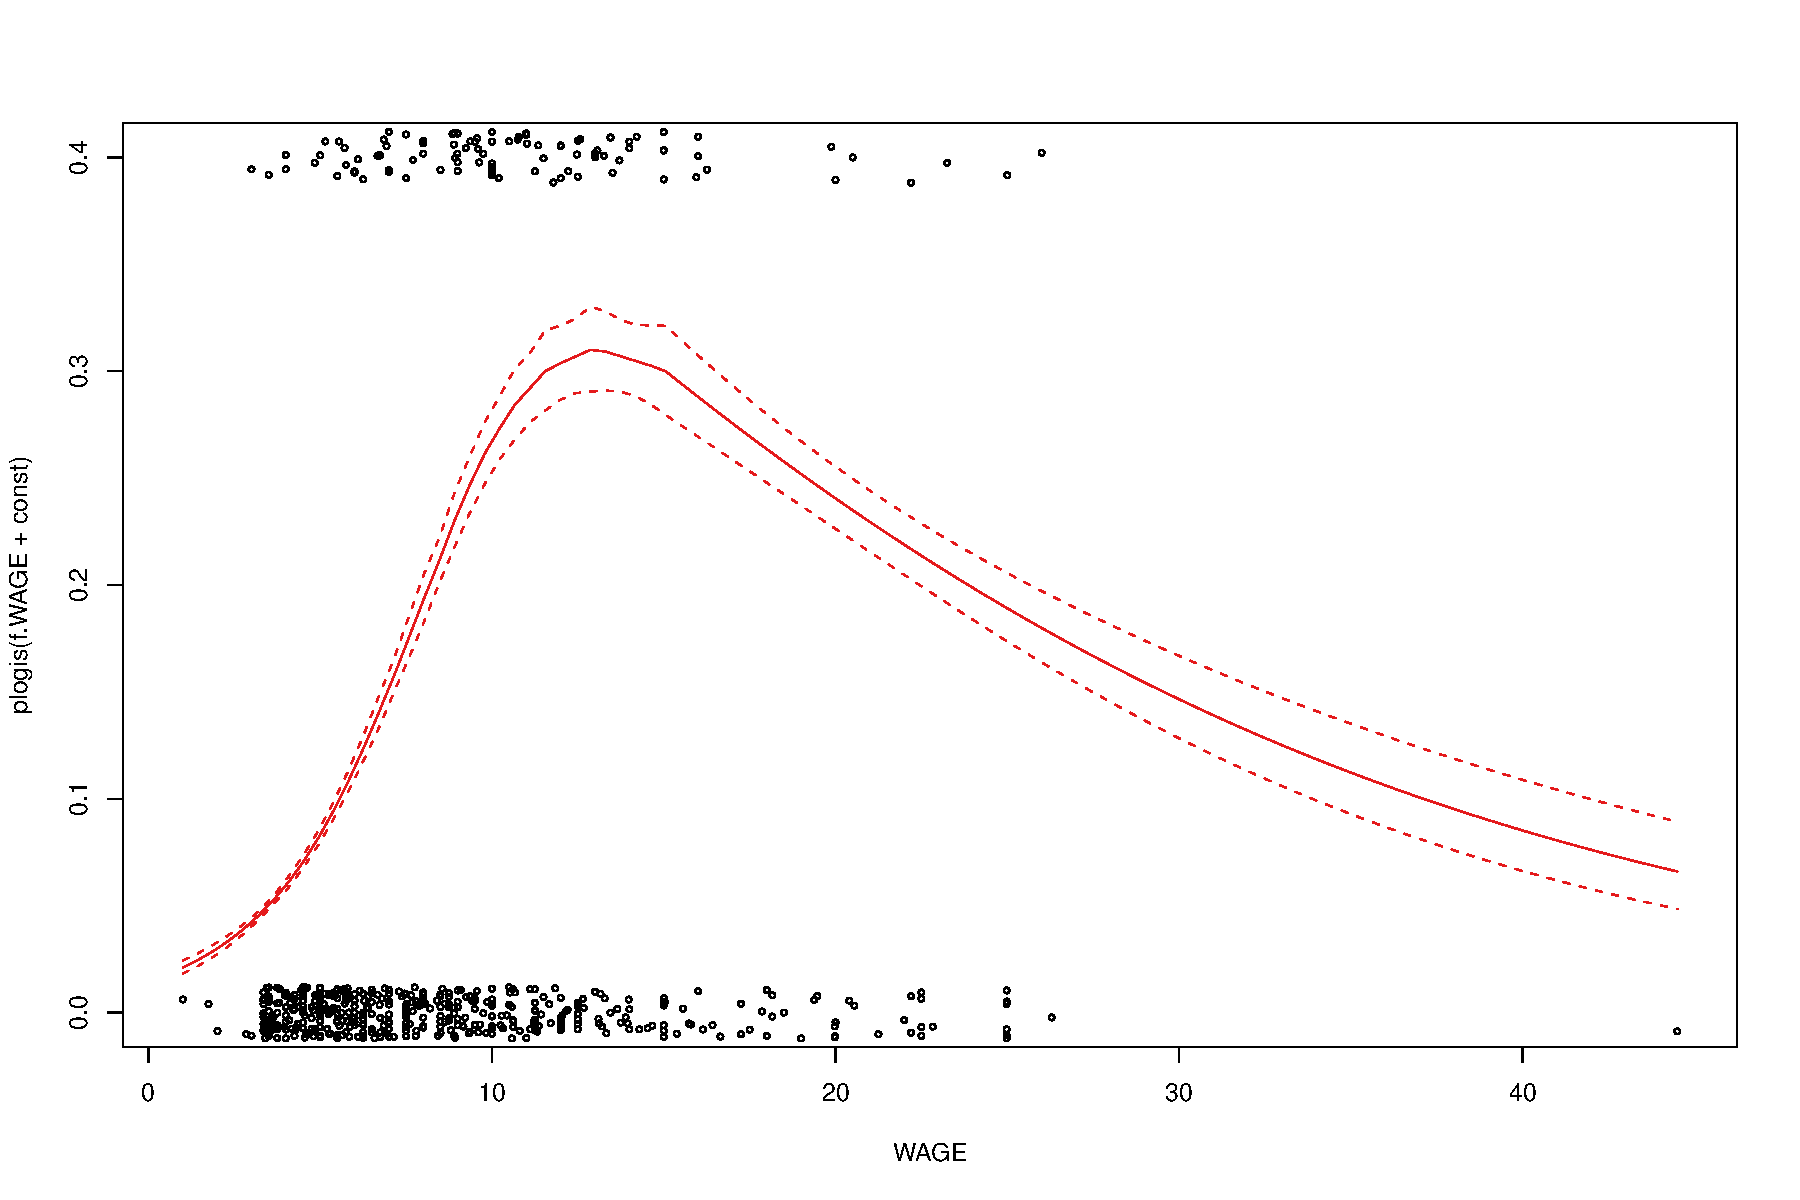
\includegraphics{GAMMsUsingLME4-unionPlot}
\caption{Fitted probability of union membership versus hourly wages, 
with conditional pointwise 90\% CI and jittered observations. \label{unionPlot}}                    
\end{center}
\end{figure}


\clearpage
\subsection{Separate smooths for levels of a factor: Using the \texttt{by}-option}\label{ExBy}
We use data on coronary sinus potassium concentration measurements for 36 dogs.
The dogs were divided into 4 treatment groups, and the measurements for each dog
were taken every two minutes from 1 to 13 minutes after occlusion (i.e. an
artificially induced heart attack). The data was first published in
\cite{Grizzle:1969} and previously analysed in \cite{Crainiceanu:2005}. 

\begin{figure}[!htbp] \centering
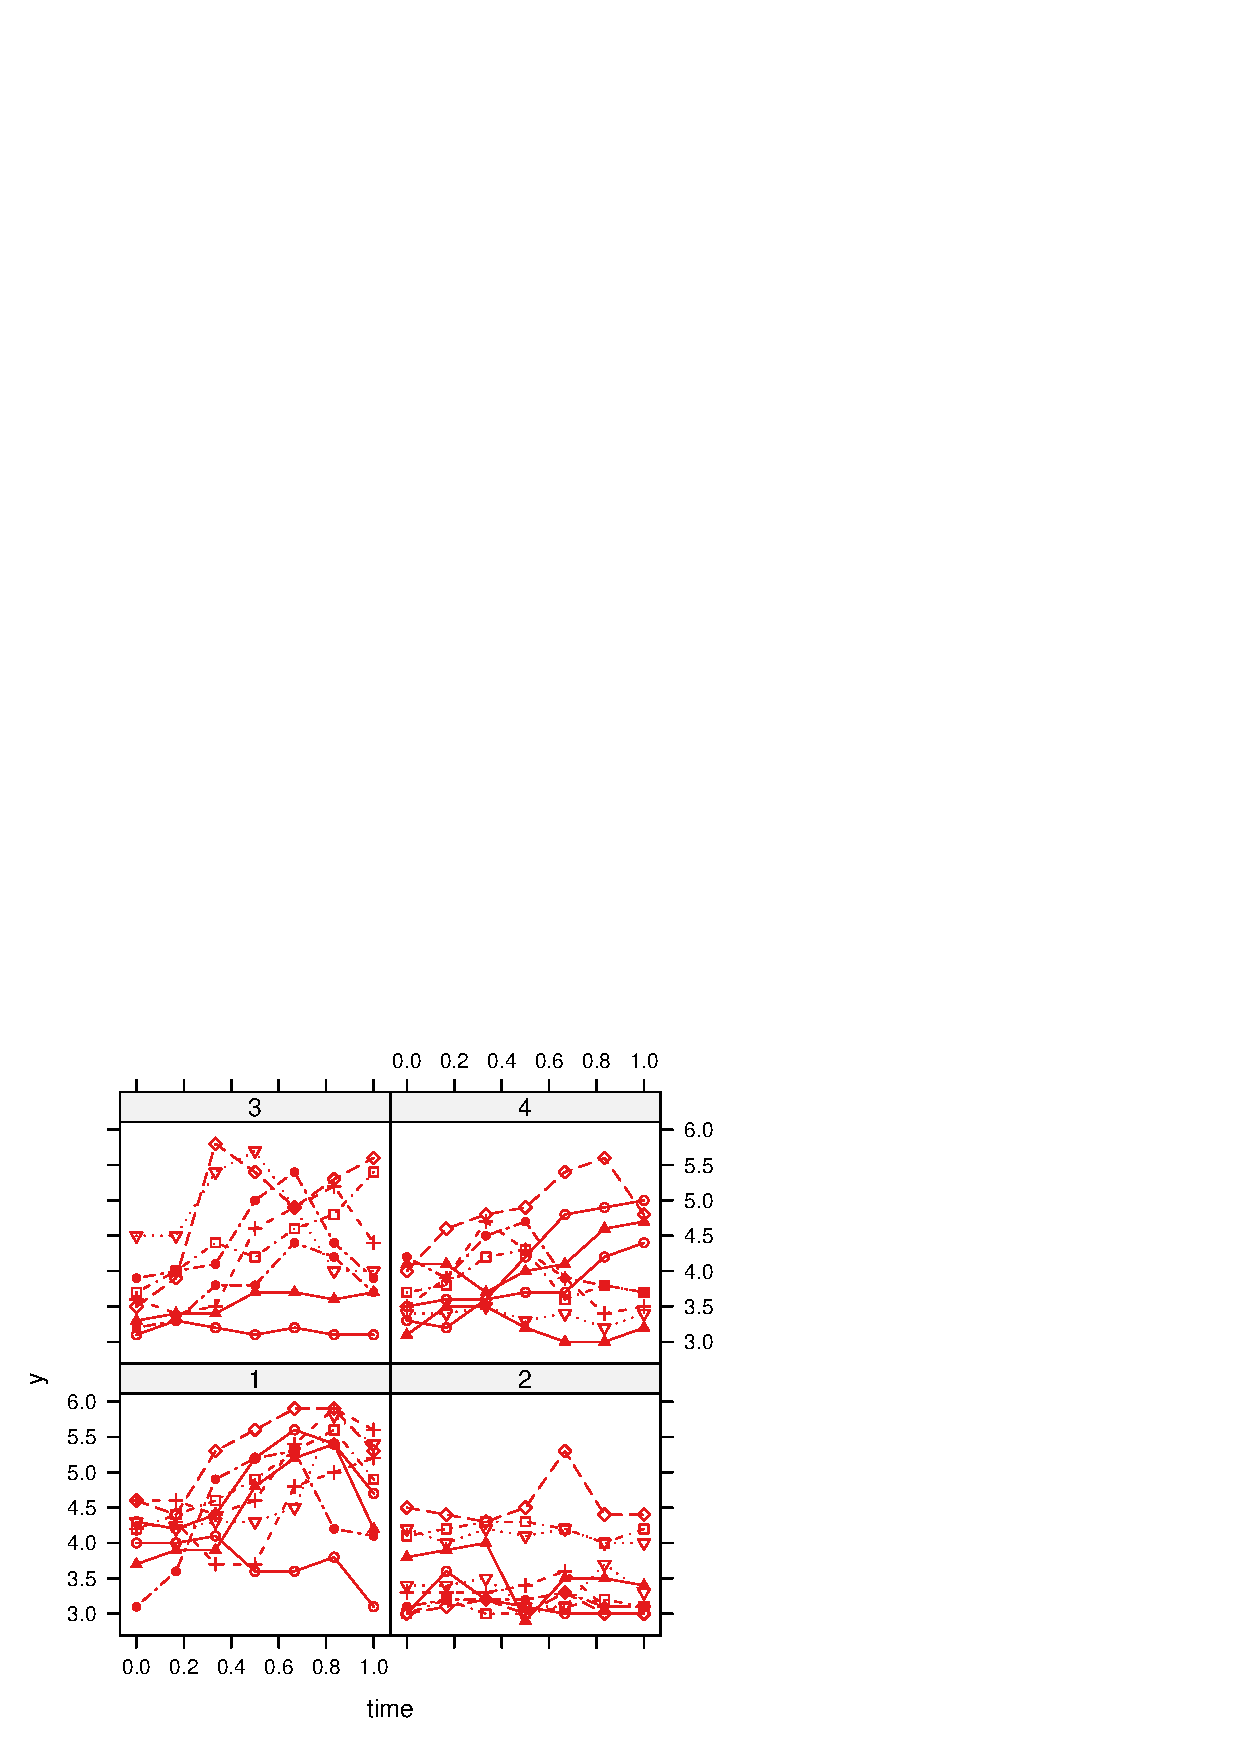
\includegraphics{GAMMsUsingLME4-dogPlot}
\caption{\code{dog} data: coronary sinus potassium concentrations for 36 dogs in 4 treatment groups\label{dogPlot}}                    
\end{figure}
Figure \ref{dogPlot} shows the observed concentrations for all 36 dogs split up into the
treatment groups. The group-averages seem to have quite different time trends,
with different degrees of nonlinearity, so we fit an additive mixed model with
group-specific smooth functions $f^g_{g(i)}(t),$ $g(i)=1,\dots,4,$ of time and random
intercepts $b_0$ for the different dogs:
\begin{align*}
y_{ij} &= \beta_{0g(i)} +  f^g_{g(i)}(t_{ij}) + b_{0i} + \eps_{ij}\\
f^g_{g(i)}(t_{ij}) &= \beta_{1g(i)} t_{ij} + \sum_{k=1}^{K-1} b^g_{g(i)k}(t_{ij}- \kappa_k)_+ \\
b^g_{g(i)k} &\sim N(0, \sigma^2_{g(i)}) \\
b_{0i} &\sim N(0, \sigma^2_{b0}) \\
\eps_{ij} &\sim N(0, \sigmaeps) 
\end{align*}
Note that we estimate different spline coefficient variances  $\sigma^2_{g(i)},\; g(i)=1,\dots,4$ 
for the 4 treatment groups.

Since there are only 8 unique time points for the measurements, 
6 knots should be enough to model the time trends.
The model is specified in \code{amer} using the \code{by}-option:
\begin{Schunk}
\begin{Sinput}
> d1 <- amer(y ~ -1 + group + tp(time, k = 6, by = group) + 
+     (1 | dog), data = dog)
\end{Sinput}
\end{Schunk}
\begin{Schunk}
\begin{Sinput}
> print(d1, corr = F)
\end{Sinput}
\begin{Soutput}
Additive mixed model fit by REML 
Formula: y ~ -1 + group + tp(time, k = 6, by = group) + (1 | dog) 
   Data: dog 
 AIC BIC logLik deviance REMLdev
 383 433   -178      341     355
Random effects:
 Groups        Name        Variance Std.Dev.
 dog           (Intercept) 0.2487   0.499   
 f.time.group4 tp          0.0119   0.109   
 f.time.group3 tp          0.1236   0.352   
 f.time.group2 tp          0.0000   0.000   
 f.time.group1 tp          0.3349   0.579   
 Residual                  0.1508   0.388   
Number of obs: 252, groups: dog, 36; f.time.group4, 5; f.time.group3, 5; f.time.group2, 5; f.time.group1, 5

Fixed effects:
                Estimate Std. Error t value
group1            4.4176     0.3828   11.54
group2            3.5529     0.1644   21.61
group3            4.3789     0.3350   13.07
group4            4.0325     0.2148   18.77
time.group1.fx1   0.2180     0.2808    0.78
time.group2.fx1  -0.0329     0.0465   -0.71
time.group3.fx1   0.5399     0.2395    2.25
time.group4.fx1   0.2187     0.1245    1.76
\end{Soutput}
\end{Schunk}
Note \code{amer}'s naming convention for smooth functions with a
\code{by}-argument: The group name of the variance component associated with a
smooth function of a covariate \code{x} at level \code{L} of the grouping factor 
\code{by} is \code{f.x.byL}. The names of the columns in the $n \times p$ design
matrix $\bm X_{u, L}$ for the unpenalized part of the smooth for level \code{L}
are given by \code{x.byL.fx1, x.byL.fx2} to \code{x.byL.fxp}.
\begin{figure}[!htbp]
The following code generates figure \ref{dogPlotBy}:
\begin{center}
\begin{Schunk}
\begin{Sinput}
> layout(cbind(matrix(1, ncol = 2, nrow = 2), matrix(2:5, 
+     ncol = 2, nrow = 2)))
> par(mar = c(3, 2.8, 2.8, 0.8), mgp = c(2, 1, 0))
> plotF(d1, ylim = range(dog$y), interval = "none", legend = "topleft", 
+     level = 0.95, auto.layout = F, lwd = 3)
> d1.RW <- getF(d1, interval = "RW")
> for (i in 1:4) {
+     plot(0, 0, ylim = range(dog$y), xlim = c(0, 1), ylab = "y", 
+         xlab = "time")
+     sub <- subset(dog, group == i)
+     lapply(split(sub, sub$dog, drop = T), function(x) lines(x$time, 
+         x$y, col = "lightgrey", lty = 1, lwd = 1))
+     matlines(d1.RW[[1]][[i]][, 1], d1.RW[[1]][[i]][, 
+         -1], type = "l", lty = c(1, 3, 3), col = i, lwd = 2.5)
+ }
\end{Sinput}
\end{Schunk}
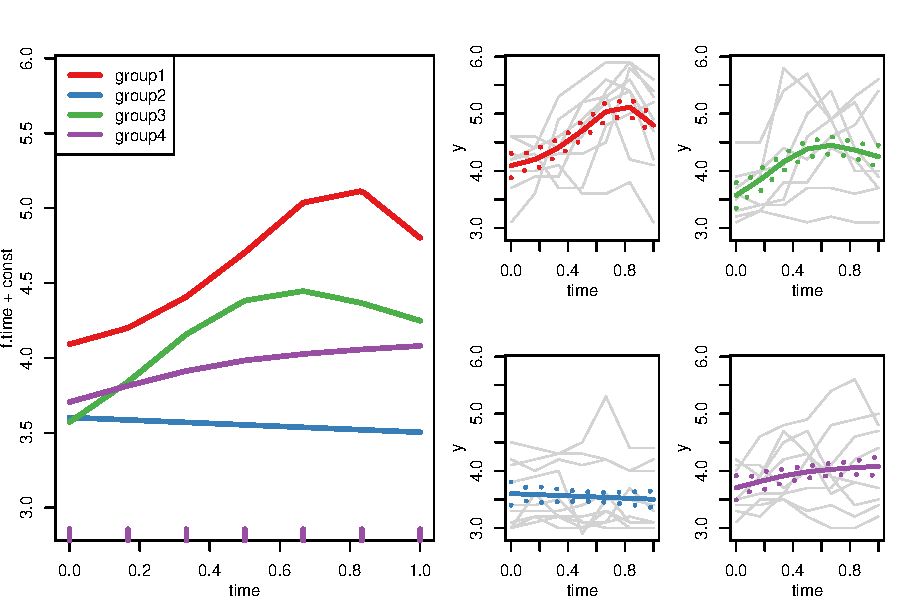
\includegraphics{GAMMsUsingLME4-dogPlotBy}
\caption{Left panel: Estimated groupwise smooths for the coronary sinus potassium data;
Right panels: Estimated groupwise smooths with pointwise 90\% CIs and observed data (grey) \label{dogPlotBy}}                    
\end{center}
\end{figure}

\clearpage
\subsection{Subject- or cluster-specific smooths: Using the \texttt{allPen}-option}\label{ExAllP}

It is also possible to allow smooth subject-specific deviations from the
group-specific curves. The model is now:
\begin{align*}
y_{ij} &= \beta_{0g(i)} +  f^g_{g(i)}(t_{ij}) + f^s_i(t_{ij}) + \eps_{ij} \\
f^g_{g(i)}(t_{ij}) &= \beta^g_{1g(i)} t_{ij} + \sum_{k=1}^{K_g} b^g_{g(i)k}(t_{ij}- \kappa_k)_+ \\
f^s_i(t_{ij}) &= b_{0i} + b_{1i} t_{ij} + \sum_{k=1}^{K_i} b^s_{ik}(t_{ij}- \kappa_k)_+ \\
b^g_{g(i)k} &\sim N(0, \sigma^2_{g(i)}) \\
b^s_{ik} &\sim N(0, \sigma^2_{fs}) \\
\left(b_{0i},b_{1i}\right)\tr &\sim N_2(\bm 0, \bm D) \\
\eps_{ij} &\sim N(0, \sigmaeps)
\end{align*}
We still estimate separate spline coefficient variances 
$\sigma^2_{g(i)},\; g(i)=1,\dots,4$
for the 4 treatment groups, but only one common spline coefficient
variance $\sigma^2_{fs}$ for all the subject-specific smooth functions $f^s_i(t)$. We assume
an unstructured covariance matrix $\bm D$ for the subject-specific random
intercepts and slopes $\left(b_{0i},b_{1i}\right)$.

The model is specified in \code{amer} by using the \code{by}-option in
combination with \code{allPen = TRUE}:
\begin{Schunk}
\begin{Sinput}
> d2 <- amer(y ~ -1 + group + tp(time, k = 6, by = dog, 
+     allPen = T) + tp(time, k = 6, by = group), data = dog)
\end{Sinput}
\end{Schunk}
\begin{Schunk}
\begin{Sinput}
> print(d2, corr = F)
\end{Sinput}
\begin{Soutput}
Additive mixed model fit by REML 
Formula: y ~ -1 + group + tp(time, k = 6, by = dog, allPen = T) + tp(time,      k = 6, by = group) 
   Data: dog 
 AIC BIC logLik deviance REMLdev
 348 408   -157      298     314
Random effects:
 Groups        Name         Variance Std.Dev. Corr  
 f.time.dog    tp           0.03503  0.1872         
 u.time.dog    (Intercept)  0.25058  0.5006         
               time.dog.fx1 0.00453  0.0673   1.000 
 f.time.group4 tp           0.01236  0.1112         
 f.time.group3 tp           0.12478  0.3532         
 f.time.group2 tp           0.00000  0.0000         
 f.time.group1 tp           0.37166  0.6096         
 Residual                   0.09315  0.3052         
Number of obs: 252, groups: f.time.dog, 180; u.time.dog, 36; f.time.group4, 5; f.time.group3, 5; f.time.group2, 5; f.time.group1, 5

Fixed effects:
                Estimate Std. Error t value
group1           4.38151    0.34252   12.79
group2           3.57606    0.17826   20.06
group3           4.33032    0.30996   13.97
group4           4.07611    0.21710   18.77
time.group1.fx1  0.18889    0.24172    0.78
time.group2.fx1 -0.00977    0.07936   -0.12
time.group3.fx1  0.50846    0.21176    2.40
time.group4.fx1  0.26291    0.12545    2.10
\end{Soutput}
\end{Schunk}
By specifying \code{allPen = TRUE}, a random intercept for the \code{by}-variable
is automatically included in the model. Also note \code{amer}'s naming convention
for smooth functions of a covariate \code{x} with a \code{by}-argument and
\code{allPen = TRUE}: For the random effects associated with $\bm X_u$, the group
name of the variance component is \code{u.x.by}. The factor \code{u.x.by} is of
course the same as \code{by}, the renaming is done for technical reasons.

Especially for spline bases with a higher dimensional nullspace of the penalty it
may not be feasible or desirable to estimate an unstructured covariance matrix
$\bm D$. By setting the \code{diag}-option to \code{TRUE} in the specification of
a smooth term with \code{allPen = TRUE}, we can enforce uncorrelated random
effects for the coefficients associated with $\bm X_u$:
\begin{Schunk}
\begin{Sinput}
> d3 <- amer(y ~ -1 + group + tp(time, k = 6, by = dog, 
+     allPen = T, diag = T) + tp(time, k = 6, by = group), 
+     data = dog)
\end{Sinput}
\end{Schunk}
\begin{Schunk}
\begin{Sinput}
> print(d3, corr = F)
\end{Sinput}
\begin{Soutput}
Additive mixed model fit by REML 
Formula: y ~ -1 + group + tp(time, k = 6, by = dog, allPen = T, diag = T) +      tp(time, k = 6, by = group) 
   Data: dog 
 AIC BIC logLik deviance REMLdev
 348 404   -158      300     316
Random effects:
 Groups        Name         Variance Std.Dev.
 f.time.dog    tp           0.0353   0.188   
 u.time.dog    time.dog.fx1 0.0000   0.000   
 u.time.dog    (Intercept)  0.1972   0.444   
 f.time.group4 tp           0.0122   0.111   
 f.time.group3 tp           0.1245   0.353   
 f.time.group2 tp           0.0000   0.000   
 f.time.group1 tp           0.3714   0.609   
 Residual                   0.0944   0.307   
Number of obs: 252, groups: f.time.dog, 180; u.time.dog, 36; f.time.group4, 5; f.time.group3, 5; f.time.group2, 5; f.time.group1, 5

Fixed effects:
                Estimate Std. Error t value
group1           4.38218    0.33499   13.08
group2           3.57596    0.16279   21.97
group3           4.33194    0.29969   14.45
group4           4.07510    0.20304   20.07
time.group1.fx1  0.18943    0.24185    0.78
time.group2.fx1 -0.00987    0.07682   -0.13
time.group3.fx1  0.50957    0.21118    2.41
time.group4.fx1  0.26190    0.12360    2.12
\end{Soutput}
\end{Schunk}

\clearpage
\subsection{Varying coefficient models: Using the \texttt{varying}-option}\label{ExVCM}

Another class of models that can be fitted with \package{amer} are
varying coefficient models. They are used to model smoothly varying
regression coefficients, i.e. models in which the effect of a
covariate $z$ varies smoothly over the range of another covariate
$x$ ($\cdot$ denotes elementwise multiplication of the columns):
\begin{align*}
\bm y &= \beta(\bm x) \cdot \bm z + \bm\eps \\
\beta(\bm x) &= f(\bm x) \approx \bm{X_u \beta +Z_p b} \\
\Rightarrow \beta(\bm x) \cdot \bm z &\approx \bm{(X_u \cdot z)\beta
+ (Z_p \cdot z) b}
\end{align*}
This class
of models can be fitted by simply scaling the design matrices for
the spline of the effect-modifying covariate $x$ (i.e. the varying
coefficient) with the values of the covariate $z$. A slight
complication arises: for all other classes of models, we drop the
intercept column in $\bm X_u$ so that the model is identifiable.
That is unnecessary in this case, so the design matrix $\bm{(X_u
\cdot z)}$ has $\bm{1 \cdot z} = \bm{z}$ as its first column.

Let's look at \package{lattice}'s \code{ethanol} data set as an example: Ethanol
fuel was burned in a single-cylinder engine. For various settings of the engine
compression (\code C) and the equivalence ratio (\code E, a measure of the
richness of the air and ethanol fuel mixture), the emissions of nitrogen oxides
(\code{NOx}) were recorded.  We assume that, for a given equivalence ratio \code E, the
relationship between compression and emissions is linear, but with different
intercepts  and slopes for different values of \code E (see figure \ref{ethanolPlot}).
\begin{figure}[!htbp] \centering
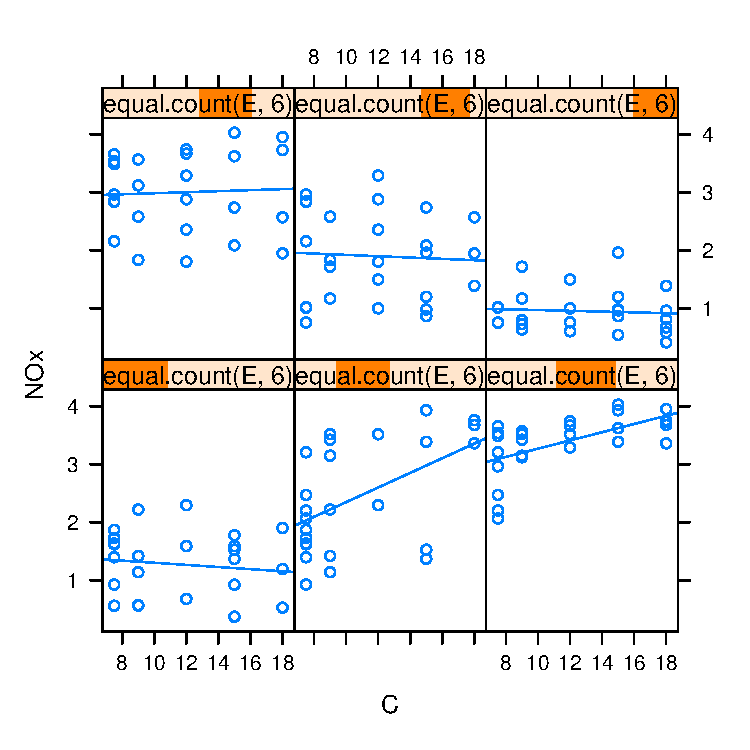
\includegraphics{GAMMsUsingLME4-ethanolPlot}
\caption{
Emissions of nitrogen oxides \code{NOx}  for various engine compression values
\code C, split up according to equivalence ratio \code E. Lines are linear
regression estimates for the subgroups.
\label{ethanolPlot}}                    
\end{figure}

The model we want to fit is
\begin{align*}
\text{\texttt{NOx}}_i &= f_1(\text{\texttt{E}}_i) + f_2(\text{\texttt{E}}_i)\text{\texttt{C}}_i + \eps_i \\
f_1(\text{\texttt{E}}) &= \beta_0 + \bm{X^{(E)}_{u}\beta^{(E)}} + \bm{Z^{(E)}_{p} b^{(E)}} \\
f_2(\text{\texttt{E}})\text{\texttt{C}} &=
\bm{X^{(EC)}_{u}\beta^{(EC)}} + \bm{Z^{(EC)}_{p} b^{(EC)}},
\end{align*}
with the usual distributional assumptions about
$\bm{b^{(E)}},\bm{b^{(EC)}}$ and $\bm\eps$. The command to fit this
model in \code{amer} is simply
\begin{Schunk}
\begin{Sinput}
> e1 <- amer(NOx ~ tp(E, k = 20) + tp(E, k = 20, varying = C), 
+     data = ethanol)
\end{Sinput}
\end{Schunk}
\begin{Schunk}
\begin{Sinput}
> print(e1, corr = F)
\end{Sinput}
\begin{Soutput}
Additive mixed model fit by REML 
Formula: NOx ~ tp(E, k = 20) + tp(E, k = 20, varying = C) 
   Data: ethanol 
  AIC  BIC logLik deviance REMLdev
 15.1 32.4 -0.554      -15    1.11
Random effects:
 Groups   Name Variance Std.Dev.
 f.E      tp   1.26248  1.1236  
 f.EXC    tp   0.00103  0.0321  
 Residual      0.02936  0.1714  
Number of obs: 88, groups: f.E, 19; f.EXC, 19

Fixed effects:
            Estimate Std. Error t value
(Intercept)   2.2834     1.0528    2.17
E.fx1         1.6808     0.7528    2.23
EXC.fx1       0.1389     0.0540    2.57
EXC.fx2       0.0317     0.0394    0.80
\end{Soutput}
\end{Schunk}
The fit is plotted in figure \ref{plotEthanolCIs}. By default, the value of the varying
coefficient function (right column) is evaluated for a covariate value of $z=1$,
so the plot for \code{f.EXC} can be interpreted directly as
$\beta(\text{\texttt{E}})$.

Note \code{amer}'s naming convention for varying coefficient models: For an effect-modifying
covariate \code{x} and an effect-causing covariate \code{z}, the function name is
given as \code{f.xXz}, the unpenalized effects are named \code{xXz.fx1} to
\code{xXz.fxp}. The first unpenalized effect corresponds to the conventional
regression coefficient for \code{z}, since $\bm{X_u}$ has $\bm{z}$ as its first
column.

\clearpage
\subsection{Variability Bands: Using the \texttt{RW}- and  \texttt{MCMC}-options}\label{VarBands}

By default, \code{amer}'s \code{plotF} computes approximate pointwise
intervals for the smooth functions based on a bias-adjusted \cite[ch. 6.4]{Semip:Regr} approximation of 
\mbox{$\Cov((\bm{\hat\beta,\hat b -b})|\hat \sigma^2_b, \hat \sigmaeps)$} (see \ref{VarEst}). 
These may underestimate the true variability since they ignore the uncertainty in the estimated variance
parameters. 

Alternatively, the results from \package{lme4}'s \code{mcmcsamp} can be used to
construct MCMC-based variability bands. Figure \ref{plotEthanolCIs} compares
the frequentist, bias-adjusted variability bands (see \ref{VarEst}) for the
estimated function values with pointwise HPD-Intervals based on 1000 draws from
\code{mcmcsamp} for the \code{ethanol} data. We expect the latter to be wider since
they take into account the variability of the estimated variances, while the
former are conditioned on the estimated variances. 
\begin{figure}[!htbp] \centering
\begin{Schunk}
\begin{Sinput}
> par(mfrow = c(2, 2), mar = c(3, 2.8, 2.8, 0.8), mgp = c(2, 
+     1, 0))
> e1.RW <- plotF(e1, addConst = c(T, F), level = 0.95, 
+     auto.layout = F)
> set.seed(12345)
> e1.MCMC <- plotF(e1, addConst = c(T, F), int = "MCMC", 
+     sims = 1000, level = 0.95, auto.layout = F)
\end{Sinput}
\begin{Soutput}
starting 1000 MCMC iterations for posterior intervals:
		... done.
\end{Soutput}
\end{Schunk}
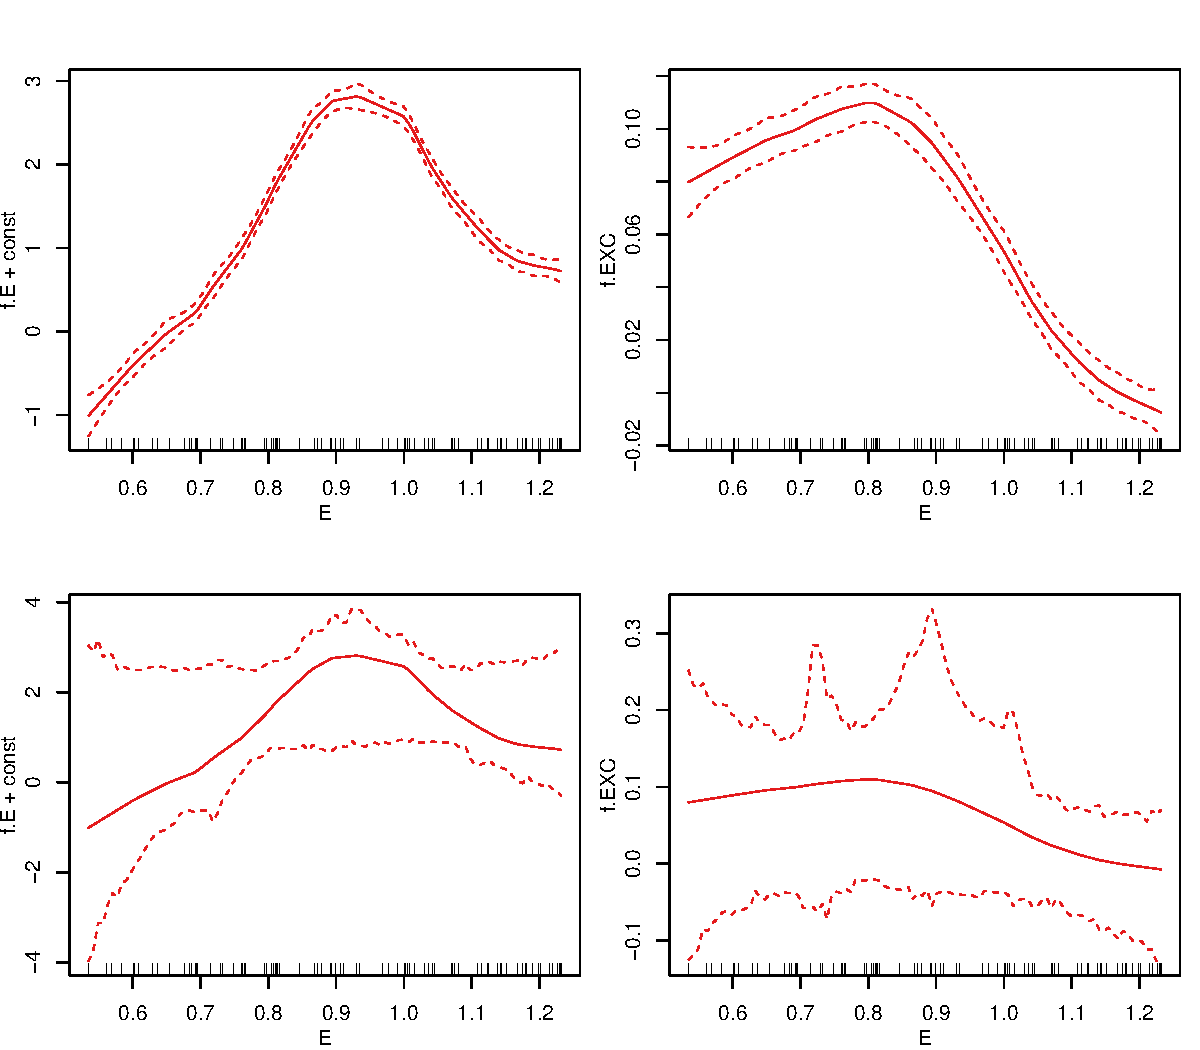
\includegraphics{GAMMsUsingLME4-ethanolCIs}
\caption{Fits and 95\% CIs/HPD-Intervals for the \code{ethanol} data.
Upper row: pointwise frequentist variability bands
conditional on the estimated variances. Lower row: pointwise HPD-Intervals based
on 1000 draws (see text) from \code{mcmcsamp}.
Left column: Effect of equivalence ratio \code{E}. Right column: 
regression coefficient for compression \code{C} varying over \code{E}.    
}\label{plotEthanolCIs}
\end{figure}

Since \code{mcmcsamp} may not always work as expected, it is strongly
recommended to examine the returned MCMC-samples. They are available as the
\code{mcmc}-attribute of the value returned by \code{getF} or \code{plotF}. A
quick visual inspection of the sampling paths can be done via \code{xyplot}, 
see figure \ref{traceplot}. The MCMC iterations in this case show strange spikes after about 700 iterations with
humongous values drawn for the relative standard deviations \code{e1@ST} of the spline
coefficients. The marginal posterior densities for the variance components are concentrated on values magnitudes larger than
the REML estimates found by the optimizer, with ridiculously long upper tails
(which lead to quite erratic sampling behaviour of the spline coefficients $\bm b$ and
consequently very broad HPD-Intervals for $\hat f(\bm x)$).
\begin{figure}[!htbp] 
\begin{Schunk}
\begin{Sinput}
> e1.MCMCData <- as.data.frame(attr(e1.MCMC, "mcmc"))
> data.frame(c(fixef(e1), e1@ST, lme4:::sigma(e1)))
\end{Sinput}
\begin{Soutput}
   X.Intercept. E.fx1 EXC.fx1 EXC.fx2   tp  tp.1 sigmaREML
tp         2.28  1.68   0.139  0.0317 6.56 0.187     0.171
\end{Soutput}
\begin{Sinput}
> apply(e1.MCMCData, 2, quantile, probs = c(0.1, 0.25, 
+     0.5, 0.75, 0.9), na.rm = T)
\end{Sinput}
\begin{Soutput}
    (Intercept)   E.fx1  EXC.fx1  EXC.fx2   ST1     ST2 sigma
10%       0.195 -0.2168 -0.01897 -0.05728   0.0     0.0 0.168
25%       1.170  0.0763  0.00539 -0.03471   0.0     0.0 0.207
50%       1.914  0.2643  0.06521  0.00906   0.0     0.8 0.273
75%       3.263  2.4638  0.14134  0.08058  31.7    89.2 0.663
90%       5.048  3.7896  0.29875  0.15520 169.3 57125.2 0.992
\end{Soutput}
\end{Schunk}
\end{figure}
\begin{figure}[!htbp] \centering
%\begin{framed}
\begin{Schunk}
\begin{Sinput}
> print(xyplot(attr(e1.MCMC, "mcmc")))
\end{Sinput}
\end{Schunk}
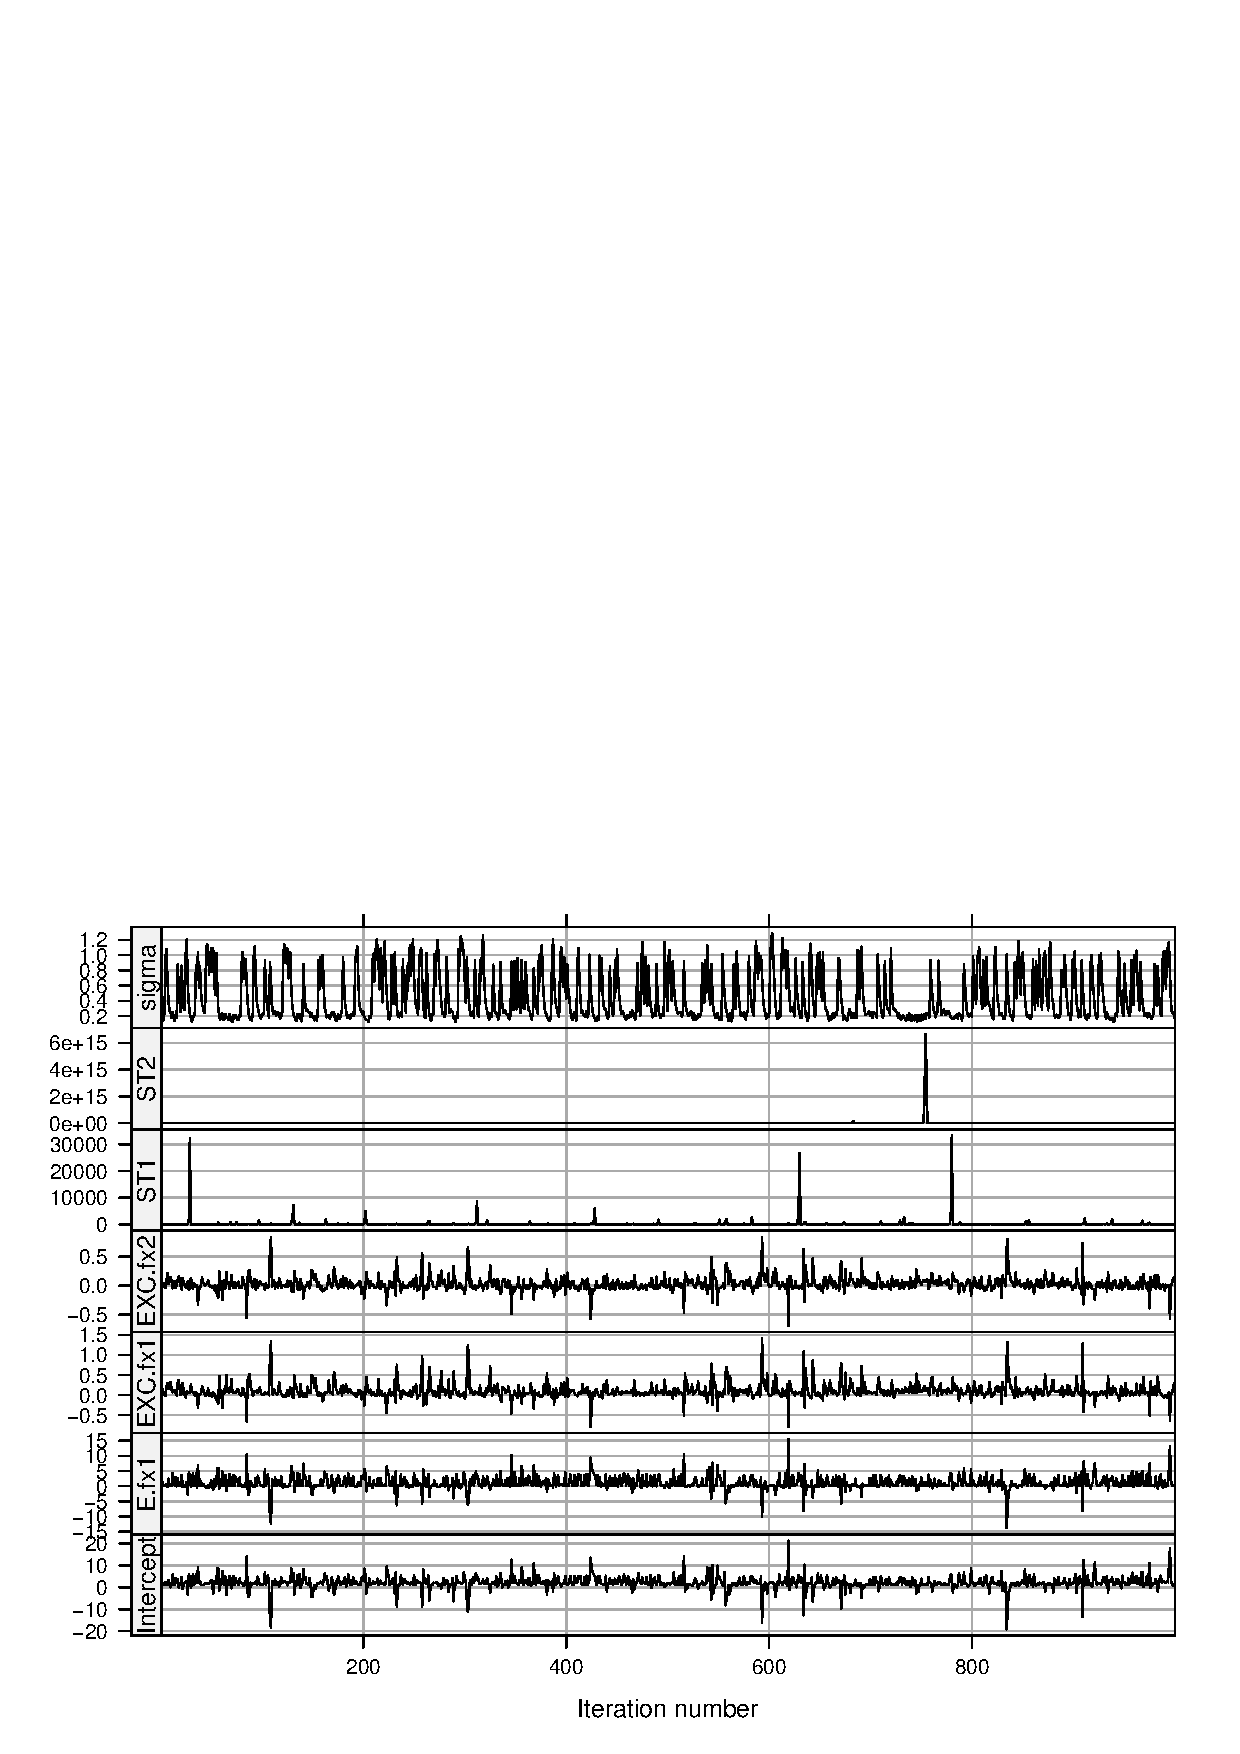
\includegraphics{GAMMsUsingLME4-ethanolMCMC}
\caption{Traceplot of the MCMC samples for model \code{e1}. Note the huge 
values for \code{ST}. \label{traceplot}}  
%\end{framed}
\end{figure}  
%<<ethanolMCMC2, echo=T>>=
%(bNormsObs <- unlist(lapply(ranef(e1.sc), function(x) sqrt(sum(x^2)))))
%bNormsMCMC <- apply(attr(e1.MCMC,"mcmc")@ranef[,1:153], 2, function(x) return( sqrt(c(sum(x[1:19]^2, na.rm=T),sum(x[20:38]^2, na.rm=T)))))
%apply(bNormsMCMC, 1, quantile, probs=c(.1, .25 ,.5, .75, .9), na.rm=T)
%@

\clearpage
\section{Implementation}

\subsection{What's the point?}
There is already a well-tested, well documented and versatile package
\package{mgcv} \citep{mgcv} that fits generalized additive mixed models in
\R, so why bother with yet another one?
\begin{itemize}
	\item \package{mgcv}'s \code{gamm} uses the less stable and slower
\package{nlme}-implementation of linear mixed models, while \package{amer} relies
on the more stable algorithm used in \package{lme4} \citep{lme4} with its very
fast sparse \package{Matrix} \citep{Matrix} magic. 
Also, specifying random effects terms for \code{amer/lmer} does not use \code{gamm/nlme}'s cumbersome list notation. 
	\item \package{mgcv}'s \code{gamm} fits non-gaussian responses by calling
\package{MASS}'s \code{glmmPQL}. The PQL-approach for fitting generalized linear mixed models
(GLMM) is severely biased and often unstable.  \package{amer} relies on the more
precise Laplace approximation implemented in \package{lme4} for fitting GLMMs.
	\item \package{asreml} also offers additive models, but is limited to gaussian
responses (and isn't free or open-source)
\end{itemize} 
The \code{/tests} file \code{mgcvTests.R} does some comparisons between \code{gamm} and \code{amer}.
The drawbacks of using \package{amer} instead of \package{mgcv}'s \code{gamm}
are that, as yet, it's not possible to include serial and/or spatial correlation
structures or variance functions for the residuals or specify covariance
structures of the random effects that aren't either diagonal or unstructured
(this will remain an issue as long as \package{lme4} doesn't have that
capability). Also, multidimensional smooths are not yet implemented, 
but will be included in a future version. 
\subsection{Making \code{lmer} fit GAMMs}
In its most current version (\texttt{0.999375-33}, at the time of writing), 
\package{lme4} fits mixed models
\begin{itemize}
\item for hierachical data structures (i.e. grouped data) and
\item only admits either diagonal or unstructured covariances of the non-scalar random 
effects for every level of grouping.
\end{itemize}

In an additive mixed model, data are not grouped (the smoothing introduces
dependence between all the observation in the data) and, if the reparameterization
from $\bm B \bm \delta$ to $\bm{X_u\beta} + \bm{Z_p b}$ is not done, the
precision matrix $\bm K / \lambda$ for the penalized coefficients is in general not
diagonal (and certainly not unstructured) and not of full rank, so that an
implementation of GAMMs based on the unreparameterized representation is not
possible without changing the underlying C-code of \package{lme4}.

Instead of making these changes to the underlying C, \code{amer} tricks
\code{lmer} into fitting additive models by setting up an unfit model object with
the structure of random and fixed effect design matrices necessary for the mixed
model representation \eqref{F:Reparam} of the additive model, and then
overwriting the (precursor of) the \code{Zt}-slots with the penalized parts $\bm
Z_p$ of the reparameterized spline bases. More precisely, the model object is set
up by going through the following steps for each smooth function:
\begin{enumerate}
\item Generate $\bm X_u$ and $\bm Z_p$ according to the basis generating
function (see section \ref{RollYourOwn}) given for the smooth term,
\item replace the smooth term in the original model formula with fixed effect terms
for the columns in $\bm X_u$ and a random intercept term for an artificial
grouping factor that has as many levels as $\bm Z_p$ has columns,
\item add the fixed effects in $\bm X_u$ and the artificial grouping factor to the
model frame, \item set up, but do not fit this model with a call to \code{lmer}
with option \code{doFit=FALSE}, and finally
\item overwrite the design matrices for the random intercept of the artificial
grouping factor with $\bm Z_p$.
\end{enumerate}
Some complications arise if the \code{by}-, \code{allPen}- or \code{varying}-options are used, but
these steps remain basically the same. The modified
unfitted model is given to \small{\verb+lmer_finalize+} or \small{\verb+glmer_finalize+}
for calling the optimization C-code.


\subsection{Why use the TP-basis?}
The following flaws of the TP-basis that is used as the default in \package{amer} are often mentioned: 
\begin{itemize}
\item it has an undesirable one-to-one mapping between the smooth\-ness/\-differen\-tiability
of the fit (TP of degree $p$ $\Rightarrow$ fit is $p-1$-time
continuous differentiable), and the nullspace of the penalty (TP of degree $p$
$\Rightarrow$ nullspace is a $p$-degree polynomial). This is different from,
e.g., penalized B-Spline fits, where the order of the difference penalty that
determines the nullspace of the penalty can be specified independently from the
order of the spline bases which determine the smoothness of the fit.
\item the unbounded support (to the right of the knot) of the truncated
polynomials means that the values of the basis function can potentially become
huge.
\item the columns in $\bm Z_p$ containing the truncated polynomials are
severely collinear, especially for closely spaced knots
\end{itemize}
Why did I use it nevertheless? 
For one, similar collinearity in $\bm Z_p$ is present for all other spline bases
I am aware of after the mixed model reparameterization \eqref{F:Reparam} described in section
\ref{Reparam}.
More importantly, for all other spline
bases I am aware of, the reparameterized design $\bm Z_p$ contains no systematic zeroes at all even if the matrix of the original basis functions $\bm B$ 
is sparse, while $\bm Z_p$ for the TP-basis is about 50\% zeroes. This means that \package{amer} can take advantage 
of the sparse matrix operations in \package{lme4} when \code{tp} or \code{tpU} is used, but not for any other bases.

\subsection{Writing your own basis-generating function}\label{RollYourOwn}

It is fairly easy to implement your own basis generating function for use in
\package{amer}. Such a function only has to fullfill the following criteria:
\begin{itemize}
\item It has to have at least the arguments 
\begin{itemize}
\item \code{x}, a \code{numeric} variable used for the smooth function,
\item \code{by}, a \code{factor} variable  (default: \code{NULL}),
\item \code{allPen}, (a \code{logical}),
\item \code{diag}, (a \code{logical}),
\item \code{varying}, a \code{numeric} variable (default: \code{NULL}).
\end{itemize}
\item It has to return a list with
\begin{itemize}
\item an entry named \code X, which contains the matrix $X_u$ without the
intercept column (this can be a matrix with zero columns) 
\item an entry named \code Z, which contains the matrix $Z_p$
\item an attribute \code{call}, which contains the result of \code{expand.call}
\end{itemize}
\end{itemize}
You don't have to worry about the reparametrization described in \ref{Reparam}
- the utility function \code{reparameterizeDesign} creates $\bm X_u$ and $\bm Z_p$ 
for a given design matrix $\bm B$ and the associated penalty matrix $bm K$.
The technical details of splitting up $\bm X_u$ and $\bm Z_p$ for a possible
\code{by} variable, naming the columns in $\bm X_u$ etc.~are performed by the
utility function \code{expandBasis}.

As an example, let's add a variant of the TP-Basis to \code{amer}'s repertoire --
let's say we want to get rid of the undesirable one-to-one mapping between the
smoothness/differentiability of the fit and the null-space of the penalty of the
TP-basis. We implement a simple basis-generating function \code{tp2} that lets us
specify the dimensionality of the nullspace so that, for a TP-spline basis of
degree $p$ without intercept (see above), we can specify the degree of the global
polynomial that is unpenalized\footnote{This basis is available im \textsf{amer} as \texttt{tpU}.}. 
Let's call this option \code{dimU}. If we set \code{dimU}$=p$, this
corresponds to the conventional TP-Penalty. If \code{dimU}$<p$, columns
containing global polynomials that would be in $\bm X_u$ for the conventional
TP-Penalty are put in $\bm Z_p$ instead.
 
The following code implements a rough draft of the idea, with the default for
using a quadratic TP-Basis ($p=2$) (s.t. the fitted function is continuously
differentiable, i.e. has no kinks) while penalizing deviations from linearity
(\code{dimU}$=1$):
\begin{Schunk}
\begin{Sinput}
> tp2 <- function(x, p = 2, k = 15, dimU = 1, by = NULL, 
+ 		allPen = FALSE, diag = FALSE, varying = NULL, 
+ 		knots = quantile(x, 
+ 			probs = (2:(k - p + 1))/(k - p + 3)))
+ {
+ 	#dim. of nullspace can't be larger than p of TP-basis:
+ 	stopifnot(dimU <= p)
+ 	
+ 	#always need this for the call attribute of the returned value:
+ 	call <- as.list(expand.call())
+ 	call$knots <- knots
+ 	
+ 	#global polynomial trends:
+ 	X <- outer(x, 0:p, "^") 
+ 	
+ 	#truncated power basis functions
+ 	Z <- outer(x, knots, "-")^p * outer(x, knots, ">")
+ 	
+ 	#matrix of basis functions 
+ 	B <- cbind(X, Z)
+ 	
+ 	#the penalty matrix K is the identity matrix, 
+ 	#	with (dimU+1)-leading zeroes
+ 	# (dimU + 1 because of the intercept column...)
+ 	K <- diag(ncol(B))
+ 	K[cbind(1:(dimU + 1), 1:(dimU + 1))] <- 0
+ 	
+ 	#let reparameterizeDesign do the dirty work
+ 	D <- reparameterizeDesign(B, K)
+ 	
+ 	#return X_u and Z_p
+ 	res <- list(X = D$X, Z = D$Z)
+ 	attr(res, "call") <- as.call(call)
+ 	return(res)
+ } 
\end{Sinput}
\end{Schunk}

We can now use this function to fit a continuously differentiable function with
penalized deviations from linearity to the dog data, but we have to tell
\code{amer} to look for smooth terms called \code{tp2} in the
\code{basisGenerators}-option:
\begin{Schunk}
\begin{Sinput}
> d4 <- amer(y ~ -1 + group + tp2(time, k = 6, p = 2, dimU = 1, 
+     by = group) + (1 | dog), data = dog, basisGenerators = c("tp2"))
\end{Sinput}
\end{Schunk}
\begin{Schunk}
\begin{Sinput}
> print(d4, corr = F)
\end{Sinput}
\begin{Soutput}
Additive mixed model fit by REML 
Formula: y ~ -1 + group + tp2(time, k = 6, p = 2, dimU = 1, by = group) +      (1 | dog) 
   Data: dog 
 AIC BIC logLik deviance REMLdev
 373 422   -172      340     345
Random effects:
 Groups        Name        Variance Std.Dev.
 dog           (Intercept) 2.49e-01 4.99e-01
 f.time.group4 tp2         1.17e-01 3.41e-01
 f.time.group3 tp2         1.47e+00 1.21e+00
 f.time.group2 tp2         1.01e-11 3.18e-06
 f.time.group1 tp2         1.85e+01 4.30e+00
 Residual                  1.50e-01 3.88e-01
Number of obs: 252, groups: dog, 36; f.time.group4, 5; f.time.group3, 5; f.time.group2, 5; f.time.group1, 5

Fixed effects:
                Estimate Std. Error t value
group1             4.215      0.481    8.76
group2             3.553      0.164   21.61
group3             4.571      0.290   15.76
group4             4.034      0.202   19.98
time.group1.fx1   -0.286      1.162   -0.25
time.group2.fx1    0.110      0.155    0.71
time.group3.fx1   -2.284      0.658   -3.47
time.group4.fx1   -0.727      0.366   -1.99
\end{Soutput}
\end{Schunk}
Figure \ref{compareTPlot} shows a comparison of the fit with 
the \code{tp2}-function to the fit of a conventional linear TP-basis.
\begin{figure}[!htbp]
The following code generates figure \ref{compareTPlot}:
\begin{center}
\begin{Schunk}
\begin{Sinput}
> par(mfrow = c(1, 2))
> plotF(d1, legend = "topleft", auto.layout = F)
> plotF(d4, legend = "none", auto.layout = F)
\end{Sinput}
\end{Schunk}
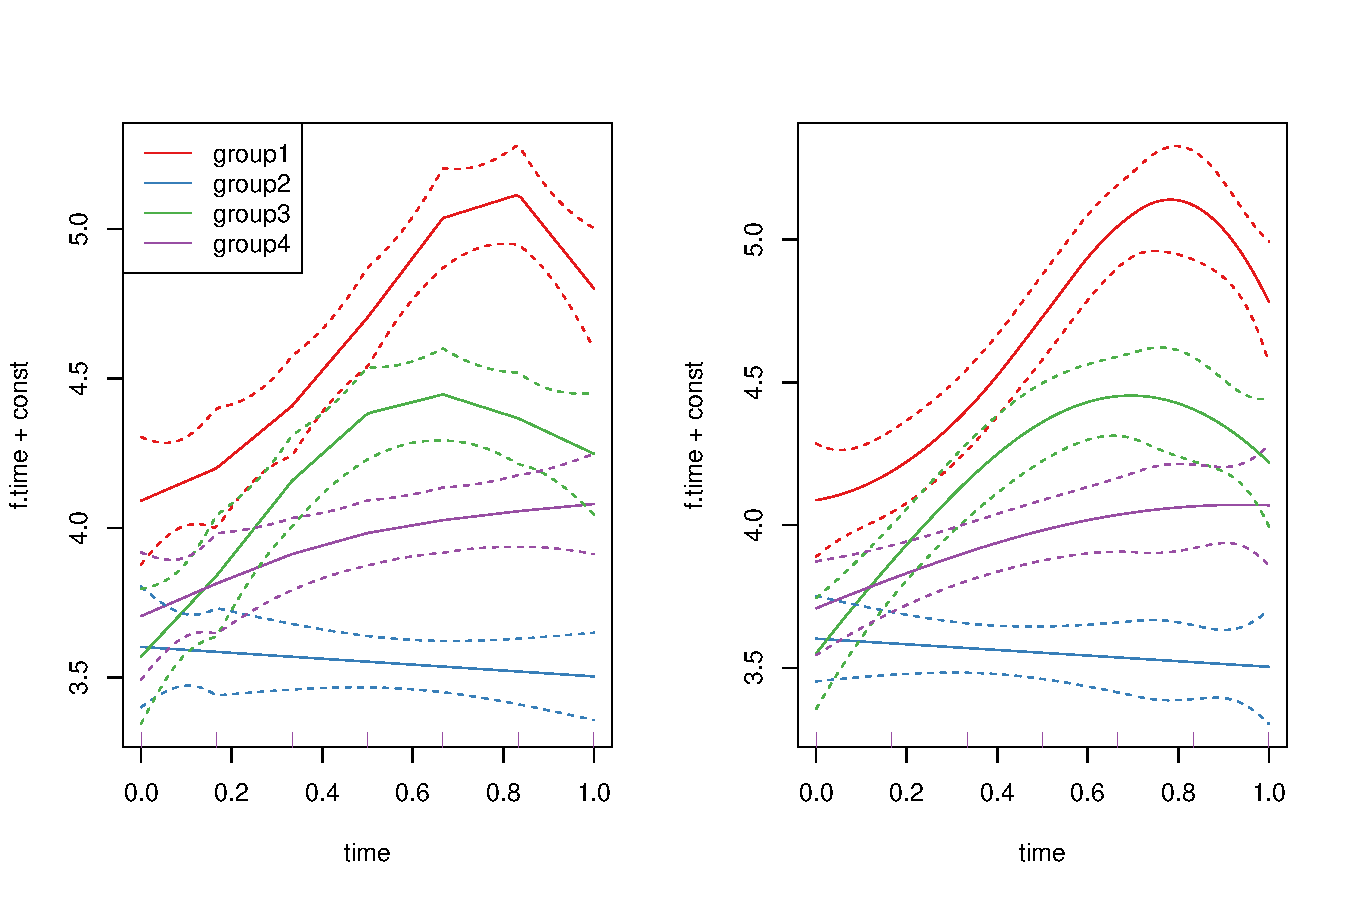
\includegraphics{GAMMsUsingLME4-compareTPTPU}
\caption{Comparison of the results for \code{tp(degree=1)} (left panel) and 
\code{tp2(degree=2, dimU=1)} (right panel) for the \code{dog} data.
 \label{compareTPlot}}
\end{center}                    
\end{figure}    
 
\clearpage 
\section{Open Issues}

A to-do list for developing \package{amer} further:
\begin{itemize}
\item approximate frequentist CI's for smooths with \code{allPen=TRUE} (should be easy, only modify \code{fctV}) 
\item 2D-smooths (will mean major re-working of most
utility functions called by \code{amerSetup} as well as \code{getF/PlotF})
\item implementing (parametric/wild/...) bootstrap-CIs 
(could use \code{lme4:::refit} and Ben Bolker's  \code{mer.sim}, maybe implement
Kauermann/\-Claeskens/\-Opsomer (2008))
\item CIs for functions based on profile likelihood methods from \code{lme4a}?
\item implementing other spline bases, e.g. for cyclic functions   
\end{itemize}

\bibliography{amer}

\end{document}



